\documentclass[tikz,border=6pt]{standalone}
\usepackage{amsmath}
\usetikzlibrary{arrows.meta,calc,patterns,positioning}
\begin{document}

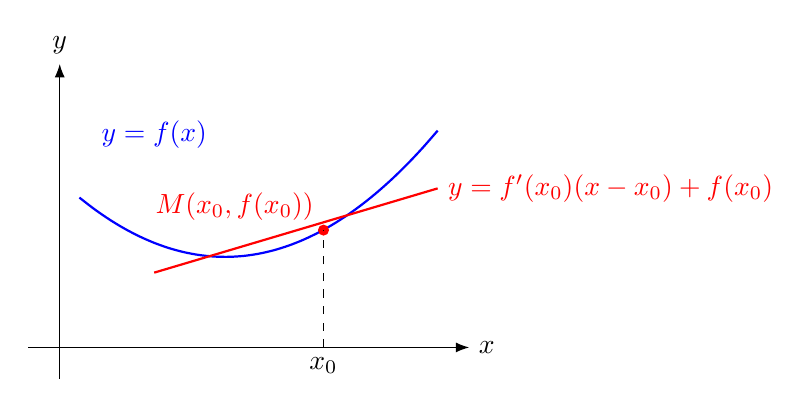
\begin{tikzpicture}[>=Latex,scale=1]
  \draw[->] (-0.4,0) -- (5.2,0) node[right] {$x$};
  \draw[->] (0,-0.4) -- (0,3.6) node[above] {$y$};
  \draw[domain=0.25:4.8,smooth,variable=\x,blue,thick] plot ({\x},{0.22*(\x-2.1)^2+1.15});
  \coordinate (A) at (3.35,1.49);
  \draw[red,thick] (1.2,0.95) -- (4.8,2.02) node[right] {$y=f'(x_0)(x-x_0)+f(x_0)$};
  \fill[red] (A) circle (2pt) node[above left] {$M(x_0,f(x_0))$};
  \draw[dashed] (3.35,0) node[below] {$x_0$} -- (A);
  \node[blue] at (1.2,2.7) {$y=f(x)$};
\end{tikzpicture}

\end{document}
